\chapter{Implementation}
\label{chap:impl}
This chapter illustrates how the proposed system is realised, i.e. deals with the implementation of the processes identified in Chapter~\ref{chap:arch}, their interfaces and the techniques used to achieve the required functionality. \\

It opens with a description of external frameworks employed in this work. The other sections reflect the structure of the architecture and follow an object from image in the database, through detection in a camera image, to the memory of the semantic map and eventually its visual representation on the computer screen.


\section{External frameworks}
\label{sec:impl-external}
This work integrates several external frameworks and programming libraries into the development of the proposed system. They provide existing solutions for some of the required capabilities. \\

The following frameworks will come up again and again over the course of this chapter, because they help with recurring, high-level functionality, e.g. communication between the various subsystems.

\subsection{ROS as an inter-process communication service}
\label{sec:impl-ros}
\begin{wrapfigure}{l}{0.33\textwidth}
  \vspace{-10pt}
  \centering
  
\includegraphics[width=0.31\textwidth]{images/Logo_ROS.png}
  \vspace{-10pt}
\end{wrapfigure}

ROS, short for ``\textbf{R}obot \textbf{O}perating \textbf{S}ystem'', ``provides a structured communications layer above the host operating systems of a heterogenous compute cluster.''\cite{quigley2009ros}. ROS implements several methods for inter-process communication and is sufficient to realize the interfaces defined in Chapter~\ref{chap:arch}. \\

Processes created with ROS are called \textbf{Nodes}. They communicate with each other through \textit{messages} and \textit{services}. The subsystems identified in the architecture description (Section~\ref{chap:arch}) are implemented as ROS nodes. \\

\textbf{Messages} can contain multiple fields of standard datatypes (e.g. \texttt{boolean}, \texttt{integer}, \texttt{float}, etc). They are used to broadcast and / or stream information to every node that might be interested. These messages are \textit{published} to a certain \textit{topic}. Other nodes can \textit{listen} to a topic, so that they will receive new information associated with it. This enables them to immediately react to messages, without needing to continuesly query a topic.

ROS is able to synchronize messages. If a node wants to listen to multiple topics at once, ROS can resolve slight differences in timing and tell if messages were published simultaneously. This practice satisfies the requirement (defined in Section~\ref{sec:arch-perception}) of being able to get the camera and depth images for the same moment of time.

\begin{lstlisting}[caption=An example for the use of ROS messages in this work. The database informs others about changes.]
/**
 * Database. The publisher.
 */
int main(int argc, char** argv) {
  // Initialize ROS
  ros::init(argc, argv, "thesis_database");
  ros::NodeHandle nh;
  // [...]
  // Inform subscribing nodes about changes
  ros::Publisher update_publisher;
  update_publisher = nh.advertise<std_msgs::Empty>(
    "thesis_database/updates",
    10
  );
  // Initialize database
  // [...]
  // Publish that the contents of the DB changed
  std_msgs::Empty msg;
  update_publisher.publish(msg);
  // [...]
}
\end{lstlisting}

\begin{lstlisting}[caption=An example for the use of ROS messages in this work. The perception reacts to changes to the database.]
/**
 * Perception. The listener.
 */
void callback(const std_msgs::Empty& input) {
  // Process changes in the database
  // [...]
}

int main(int argc, char** argv) {
  // Initialize ROS
  ros::init(argc, argv, "thesis_perception");
  ros::NodeHandle nh;
  // [...]
  // Subscribe to updates about the database
  ros::Subscriber database_update_subscriber;
  database_update_subscriber = nh.subscribe(
    "thesis_database/updates",
    1,
    callback
  );
  // [...]
}
\end{lstlisting}

Two-way communication in ROS is done via \textbf{services}, which basically consist of two messages. Nodes can \textit{advertise} services to enable others to \textit{request} information. The advertising node is \textit{called} with a request defined in one message and \textit{replies} to the caller with a second message.

Services are used in this work to make the information stored in the database (Section~\ref{sec:arch-db}) and semantic map (Section~\ref{sec:arch-map}) available on demand.

\begin{lstlisting}[caption=An example for the use of ROS services in this work. The semantic map enables others to get memorized objects.]
/**
 * Semantic Map. The advertiser.
 */
int main(int argc, char** argv) {
  // Initialize ROS
  ros::init(argc, argv, "thesis_mapping");
  ros::NodeHandle nh;
  // [...]
  // Advertise services
  ros::ServiceServer srv_all = nh.advertiseService(
    "thesis_mapping/get_all",
    get_all
  );
  // [...]
}
\end{lstlisting}

\begin{lstlisting}[caption=An example for the use of ROS services in this work. The visualisation gets all objects memorized by the semantic map.]
/**
 * Visualisation. The caller.
 */
int main(int argc, char** argv) {
  // Initialize ROS
  ros::init(argc, argv, "thesis_visualization");
  ros::NodeHandle nh;
  // [...]
  // Wait for the semantic map to advertise the service
  ros::service::waitForService(
    "thesis_mapping/get_all",
    -1
  );
  // Get all objects from semantic map
  ros::ServiceClient srv_client;
  srv_client = nh.serviceClient<thesis::MapGetAllSrv>(
    "thesis_mapping/get_all"
  );
  thesis::MapGetAllSrv map_get_all_service;
  if(srv_client.call(map_get_all_service)) {
    // Process objects from the semantic map
    // [...]
  } else {
    // Handle error
    // [...]
  }
  // [...]
}
\end{lstlisting}

ROS nodes can access configuration parameters stored at the \textbf{Parameter Server}. The Parameter Server supports various standard datatypes, such as \texttt{boolean}, \texttt{integer}, \texttt{float}, \texttt{string}, etc. Parameters can be defined globally, i.e. accessible by all nodes, or private, i.e. only accessible by a specific node. They can be set and retrieved in multiple ways: From within a node (i.e. via program code), with the \textit{rosparam} command-line tool, as arguments when running a node from the command-line or in \textit{.launch-files}. \\

\textbf{.launch-files} are used to as launch-``scripts'', to simplify the startup of more complex ROS systems that require multiple parameters to be set or consist of multiple individual nodes. They utilize the XML-syntax and run an arbitrary number of nodes with an arbitrary number of parameters. .launch-files are used in this implementation to start the various parts of the system, Database, Perception, Semantic Map and Visualisation at once, and to configure them to run on different devices, i.e. a robot or a standalone RGB-D camera. For example, the topics that provide the camera images and depth information might differ from device to device, therefore they can be set as parameters. Then, .launch-files are created with presets for the most common devices.

\subsection{OpenNI as the RGB-D camera driver}
\label{sec:impl-openni}
\begin{wrapfigure}{l}{0.33\textwidth}
  \vspace{-10pt}
  \centering
  
\includegraphics[width=0.31\textwidth]{images/Logo_OpenNI.png}
  \vspace{-15pt}
\end{wrapfigure}

OpenNI~\cite{openni_sdk} (``\textbf{Open} \textbf{N}atural \textbf{I}nteraction'') is a non-profit organization that provides a framework for 3D sensing. It includes drivers for RGB-D cameras, like the Microsoft Kinect, that are required by the perception (see Section~\ref{sec:arch-perception}) to recognize objects and calculate their 3D position. \\

This work uses a wrapper for the OpenNI camera driver that is available for ROS (described in Section~\ref{sec:impl-ros}). Once the package is started, it publishes the information perceived by the various sensors (RGB camera, laser sensor) of the device as well as a description of its characteristics (resolution, camera matrix, etc) to multiple ROS topics. For example, RGB color images are provided as well as grayscale images, each available raw from the device or rectified (without the distortion introduced by the lense of the camera). The same is true for the depth images created from the laser sensor, which are additionally available aligned to the camera images.

The perception requires a camera image, a depth image and the camera metadata. The specific topics can be adjusted by the user, who might not work with the defaults (depending on his device). In order to correctly recognize objects, the depth images need to be aligned with the camera images (to look up the associated depth value) and both images need to be rectified (to project pixels to 3D camera space). Note that \textit{depth registration} needs to be activated for the ROS OpenNI driver to provide these aligned images.

\subsection{The OpenCV image manipulation library}
\label{sec:impl-opencv}
\begin{wrapfigure}{l}{0.25\textwidth}
  \vspace{-10pt}
  \centering
  
\includegraphics[width=0.23\textwidth]{images/Logo_OpenCV.png}
  \vspace{-20pt}
\end{wrapfigure}

OpenCV~\cite{opencv_library} (``\textbf{Open} Source \textbf{C}omputer \textbf{Vision}'') is a library of image manipulation tools aimed at real-time computer vision development.

OpenCV not only provides implementations of popular image processing algorithms for tasks like image segmentation, object recognition and 3D reconstruction, but also a broad range of mathematical datatypes and functions for calculations in 2D and 3D cartesian coordinate systems (point, vector and matrices operations, etc).

Additionally, OpenCV comes with GUI tools and image editing functions, for example to draw points or lines onto existing images. The perception module uses these tools to visualize its results with debug images.


\section{Database}
\label{sec:impl-db}
The database is a collection of objects that are or might become interesting to the task of a robot. The system will watch out for the objects that are defined here and memorise them for future use. \\

Each entry at least has name and a sample image, i.e. a photo of the object, so the perception knows what it looks like. To create new entries to the database, other nodes (see Section~\ref{sec:impl-ros}) can provide images through the interfaces defined in Section~\ref{sec:arch-db}. These are realised with ROS services, where the requests contain contain the information to be added to the database, and the response is simply left empty.

The interfaces that allow other nodes to access objects in the database are implemented as ROS services as well.

Furthermore, the database advertises a ROS topic for updates about its content. Whenever new entries are added, it publishes a notification to this topic, which is realized as an empty ROS message. When other nodes receive this notification, it is up to them to react to the update and retrieve a new list of objects. \\

In addition to the interfaces to other nodes, the database can be provided with a path to an image directory on startup. The database will then be initialized with the images from the given directory. \\

The database deals primarily with holding information to be used by other nodes. Still, a few things need to be considered to make things easier for the perception, which will be explained briefly in the remainder of this section.

\subsection{Image size limits when adding entries to the database}
\label{sec:impl-db-limits}
Before accepting new entries, the database performs are few checks regarding the image size:

Very small images do not contain any useful information and will not be added to the database. Similarly, very large images take longer to process but might not contain any extra information that can be used by the perception. The reason for this is, that the additional information contained in sample images larger than the camera resolution can never be contained in a camera image. Instead of rejecting large images, the database determines the highest reasonable size while retaining their aspect ratio and resizes them accordingly.


\section{Perception}
\label{sec:impl-perception}
The perception is responsible for detecting the objects defined in the database, calculating the corresponding approximate 3D poses and dimensions and providing other nodes (see Section~\ref{sec:impl-ros}) with these findings. \\

To this end, it receives information from an OpenNI device (see Section~\ref{sec:impl-openni}). The necessary interface defined in Section~\ref{sec:arch-perception} is implemented through ROS messages: It listens to three different topics (camera images, depth images and camera characteristics) in sychronization, enabling it to relate the individual pieces to one another.

It then in turn publishes its calculations (the object pose, the object dimensions and the camera pose from where the objects was detected) to three different ROS topics. Other nodes can listen to these topics individually or synchronize them, e.g. to relate an object pose to the camera pose that enabled its detection. Note that all objects recognized in one camera image are published at once, so that subscribing topics know they belong to the same frame. \\

This section details what happens in between these interfaces, the way from camera image to 3D pose: The methods employed to detect objects in a fast and stable manner and the math applied to calculate its position and orientation.

\subsection{SIFT Feature Detection and Matching}
\label{sec:impl-sift}
In order to recognize objects, the perception module compares photos of them with images from the OpenNI camera (described in Section~\ref{sec:impl-openni}). A pattern of pixels in the camera image that is similar to the photo of an object is evidence for the existence of such an object. Looking for the complete photo at each possible position in the camera image in each possible size and orientation would add up to a huge amount of comparisons and is therefore unfeasible. \\

Instead, the perception uses the SIFT~\cite{sift_lowe} (Scale Invariant Feature Transform) method to detect and match local features in the objects photos and camera images. The basic idea behind local image features is to reduce the number of points of an image for further processing by selecting the points that hold the most information. Here it is used to intelligently select a significantly reduced number of points to match between the images up for comparison.

SIFT features are invariant to translation, rotation and scaling and robust under lighting changes. This means, that objects do not need to stand perfectly upright or be illuminated brightly in order to be successfully recognized.

A popular implementation of SIFT is included in OpenCV (see Section~\ref{sec:impl-opencv}).\\

The process of matching two images with SIFT consists of four steps: (1) Detecting the locations of features in both images, (2) computing a set of descriptors for each of those features, (3) calculating the distance between the descriptors of each feature in one image and the descriptors of each feature in the other image and (4) matching the features of both images by utilizing these distances.

Since the objects that are stored in the database are rarely modified, the keypoints and descriptors for their images can be stored once they are computed until the database signals a change. This means that, after a setup phase, step (1) and (2) only need to be performed for the camera image.

Similarly, computation of keypoints and their descriptors for the camera image only needs to be done once per frame. If their are multiple sample images that need to be matched against the camera image, then its keypoints and descriptors can be re-used in the matching process of all of those samples.

To determine if a feature $f$ in one image matches a feature in the other, the distance of $f$ and its nearest neighbour $f_{1st}$ should be below a threshold $t_1$. Additionally, as presented by SIFT author David G. Lowe in the succeeding paper ``Distinctive Image Features from Scale-Invariant Keypoints''~\cite{image_features_lowe}, the ratio between the distances of $f$ and its nearest neighbour $f_{1st}$ and second nearest neighbour $f_{2nd}$ in the other image can be calculated to reduce the number of false positives. If this ratio is below a threshold $t_2$, $f_{1st}$ is a match for $f$. The concept here is, that $f_{1st}$ only is a distinct, meaningful feature, if it is dissimilar to other features. \\

Step (3), comparing the descriptors of both images, is a very expensive operation. Although step (1) significantly reduces the number of points to match, it is still of quadratic complexity. In order to speed up the matching, the perception module utilizes SiftGPU~\cite{siftgpu07wu}, a SIFT implementation for the GPU. The GPU (Graphics Processing Unit) is a processor specifically designed to execute geometrical operations and image manipulation. GPUs typically consist of multiple cores that operate in parallel, further increasing performance. \todo{reference describing GPU}

One of the reasons to choose SiftGPU over other SIFT implementations for the GPU is, that its datatypes are easily interchangeable with OpenCV. This has actually been done before - the RGBD~SLAM~\cite{endres10rgbdslam} package for ROS includes a SiftGPU wrapper class that converts between SiftGPU and OpenCV. This class served as a basis for the SiftGPU wrapper classes created for this work.

Note that the SiftGPU matching process includes step (3) and (4), while they have to be done seperately when using SIFT from the OpenCV libraries.

\begin{lstlisting}[caption=Example of calculating matching points between two images with the OpenCV SIFT implementation.]
example_sift(cv::Mat& camera_img, cv::Mat& sample_img)
{
  // Feature detection
  cv::SiftFeatureDetector sift_detector;
  std::vector<cv::KeyPoint> camera_keys, sample_keys;
  sift_detector.detect(camera_img, camera_keys);
  sift_detector.detect(sample_img, sample_keys);
  // Compute descriptors
  cv::SiftDescriptorExtractor descriptor_extractor;
  cv::Mat camera_descriptors, sample_descriptors;
  descriptor_extractor.compute(camera_img,
    camera_keys, camera_descriptors
  );
  descriptor_extractor.compute(sample_img,
    sample_keys, sample_descriptors
  );
  // Calculate distances
  // between two sets of descriptors
  // (find the k=2 nearest neighbours)
  std::vector<std::vector<cv::DMatch> > matches;
  cv::FlannBasedMatcher flann_matcher;
  flann_matcher.knnMatch(sample_descriptors,
    camera_descriptors, matches, 2
  );
  // Filter matches by ratio of
  // nearest and second nearest neighbour distance
  for(size_t i = 0; i < matches.size(); i++) {
    double ratio
      = matches[i][0].distance
        / matches[i][1].distance;
    if(ratio < knn_1to2_ratio) {
      matches_filtered.push_back(matches[i][0]);
    }
  }
}
\end{lstlisting}

\subsection{Locating the 2D object position and discarding wrongly recognized objects}
\label{sec:impl-2Dpose}
If enough matching keypoints are found, the object can be located in the camera image. The matches can be used to approximate a projection from the sample to the camera image. This is done by finding a projection that transforms all matching keypoints from their sample image coordinates to their camera image coordinates. The more matches are found, the better the approximation. False positives on the other hand distort the result.

Although matches are filtered in order to reduce the number false positives (see Section~\ref{sec:impl-sift}), occasionally enough errors might come through to result in a wrongly recognized object. The perception module takes precautions to identify and discard such failures: \\

Because the scenario deals exclusively with rectangular objects, the corners of an object should form a convex quadrangle after they have been projected onto the camera image. This means that, (1) no two opposing sides of an object should intersect and (2) all four corners should be part of their convex hull. Otherwise the object can be discarded. \\

The convex hull of an object is the smallest outline one could draw around the object without a concave curvature. An algorithm to calculate the convex hull $C$ for a set of points $P = \{p_0, p_1, \dots, p_n\}$ with a complexity of $O(n * \text{log}_n)$ is the Graham~Scan~\cite{graham_scan}. The Graham Scan consists of three steps: (1) Finding a starting point, (2) sorting the other points and (3) checking for each other point, if it is part of the convex hull.

The starting point $s$ is an arbitrary point in $P$ that is part of the convex hull. One point that is definitely part of the convex hull is the point with the lowest $y$-value. If there are multiple points with the same lowest $y$-value, then the one with the lowest $x$-value of those points is definitely part of the convex hull.

After finding a starting point, the remaining points $P' = P \setminus s$ are sorted according to the angle between the $x$-axis and the line defined by $s$ and the respective point.

Finally, the algorithm traverses the sorted set of points $P'' = \text{sort}(P')$ in order to determine which points are part of the convex hull $C$. The convex hull initially is $C = \{p''_0, p''_1\}$. For each other point $p''_i$ with $i >= 2$, the last points added to the convex hull are removed, until $p''_i$ is located left of the line defined by the last and second to last points added to the convex hull. Then, $p''_i$ is added to the convex hull and the algorithm continues with $p''_{i+1}$.

To check if a point $p$ is left of a line $\overline{a b}$, a determinant
\begin{equation*}
  d = (b_x - a_x) \cdot (p_y - a_y) - (p_x - a_x) \cdot (b_y - a_y)
\end{equation*}
can be calculated. If $d > 0$, then $p$ is left of $\overline{a b}$.\\

\begin{lstlisting}[caption=This C++ code example demonstrates how the Graham Scan algorithm determines the convex hull of an already sorted set of points.]
convex_hull.push_back(p0);
convex_hull.push_back(nonP0[0]);
for(size_t i = 1;
    i < nonP0.size() && convex_hull.size() > 1; )
{
  // det2f() is
  // < 0, if C is right of AB
  // = 0, if C is on AB
  // > 0, if C is left of AB
  if(det2f(convex_hull[convex_hull.size()-2],
           convex_hull.back(),
           nonP0[i]) > 0)
  {
    convex_hull.push_back(nonP0[i]);
    i++;
  }
  else
  {
    convex_hull.pop_back();
  }
}
\end{lstlisting}

\subsection{Recognizing multiple objects of the same type by cutting successfully matched keypoints}
\label{sec:impl-multiple}
Matching multiple sample images against a camera image as described in Section~\ref{sec:impl-sift} will successfully recognize different objects in the same frame, but often multiple objects of the same type might be visible. Due to the nature of how a supermarket is organised, in a scenario as proposed in this work objects of one type always appear in groups. Matching one object against the same camera image will always return the same set of keypoints that are the best match between both images. \\

The solution to this problem is to create a subset of keypoints and descriptors for the camera image whenever an object is successfully recognized. This subset should only contain the keypoints and descriptors that do not belong to an already recognized object. Then the currently recognized object can be matched against the resulting subset again, in order to find a second best match (if such a match exists). \\

The set of keypoints associated with an object through the matching process in Section~\ref{sec:impl-sift} might contain noise, i.e. keypoints that do not belong to the object that is being matched. It also might not contain all keypoints that belong the object. Thus, another approach to create the subset of keypoints that truly belong to a recognized object is needed.

After locating the object in the camera image, it is possible to determine which keypoints are located insided the convex hull of the object and which are located outside of it. First, the points that are part of the convex hull need to be determined. Then, all the remaining points that are located left of all sides of the convex hull (when traversing the convex hull counter-clockwise) lie inside of it and all other points lie outside. To this end, the techniques introduced in Section~\ref{sec:impl-2Dpose} can be used.

The keypoints that are located outside the convex hull of a recognized object do not belong to this object. They therefore are the ones that need to be considered when looking for the second best match. This process can be repeated until no further matches for an object are found. \\

Another benefit to this method is, that successfully matched keypoints do not need to be considered when matching other objects to the camera image. On the other hand, the keypoints that are left have to be compared with the recognized object again. In most cases, the operations saved while trying to recognize the remaining objects outweigh the additional operations necessary to check for already recognized objects again, though. This depends on the number of objects that have not yet been matched against the camera image. The earlier an object is recognized, the more matching processes benefit from cutting the associated keypoints.

\subsection{Using multiple levels of detail to reduce the initial number of features}
\label{sec:impl-mipmap}
As mentioned in Section~\ref{sec:impl-sift}, keypoints and their descriptors for the camera image only need to be computed once per frame. This saves a few operations, but the matching process, which is of quadratic complexity and therefore the more expensive task, still needs to be done for every object in the database. In order to speed it up, the number of keypoints / descriptors that have to be compared can be reduced. \\

One way to cut down on necessary comparisons is to not consider successfully matched keypoints / descriptors when looking for further objects (already detailed in Section~\ref{sec:impl-multiple}). However, this method only works if an object indeed has been successfully recognized and the benefit depends on whether this object was one of the first to be processed and how much space it takes up in the camera image (i.e. how many keypoints / descriptors can be removed). \\

A more effective approach is to reduce the overall number of keypoints found by the SIFT algorithm. The OpenCV SIFT implementation and SiftGPU both offer a parameter to limit the maximum amount of features. But the increase in speed comes with the drawback of inferior quality and stability, because a lower number of keypoints results in a worse approximation of the projection from image to camera coordinate space (as described in Section~\ref{sec:impl-2Dpose}) or might not be enough to always detect an object all.

As a solution, the proposed system works with two levels of detail: First, all images are processed using only a small maximum number of keypoints. Then, if an object is successfully detected, its sample image and the camera image are matched with higher accuracy, i.e. a an increased amount of features. This way, only the objects that might actually be visible allocate the full processing power needed to locate them correctly.

Furthermore, the number of keypoints needed to be matched during the second run can be decreased by calculating a rough location of the object using the result of the first run. This location can be employed as a mask, to filter the features found using the SIFT algorithm with a higher limit (the same way keypoints are filtered in Section~\ref{sec:impl-multiple} to find multiple objects of the same type). Although such a mask is not perfect (otherwise a second run would not be necessary), the ratio of useful to useless keypoints actually increases, because only those in close proximity to the object get through, while the wider surrounding is ignored completely.

A second level of detail solves the quality issue of the perceived object location introduced by using a lower number of keypoints. But, since a rough but successful detection is needed to trigger a more precise run, stability is still a problem. To prevent loosing a visible object when the first pass was unsuccessful, a rudimentary tracking is applied: The location calculated in one frame is added for further investigation in the second run of the next frame. This can be done without increasing the workload, because successfully matched keypoints are not considered during the same frame again (see Section~\ref{sec:impl-multiple}). \\

Deciding on a maximum amount of keypoints is tricky: The right balance between keeping enough information and getting rid of unnecessary work has to be found. Also, each limit works better in some situations than others, thus a fixed number is never a definitive solution. A better way to reduce how many keypoints SIFT can find is to reduce the size of the images processed in the first pass. When scaling down an image, it looses its less distinctive features (because they are not visible anymore at a smaller size) but the amount of remaining distinctive features is not capped by a hard limit. Due to SIFTs property of being scale invariant, the remaining keypoints do not decrease in utility.

\subsection{Calculating the 3D pose of a recognized object}
\label{sec:impl-3Dpose}
Calculating the 3D pose of an object requires (1) the projection to transform points from an objects sample image to the camera coordinate space (calculated in Section~\ref{sec:impl-2Dpose}), (2) the depth image for the current frame and (3) the geometric model for the camera that is being used. The depth image and the camera model both can be obtained from the OpenNI camera (see Section~\ref{sec:impl-openni}. \\

2D image coordinates can be transformed into 3D camera space by applying the pinhole camera model (see figure~\ref{fig:pinhole-camera}) with the camera characteristics obtained via the OpenNI driver (see Section~\ref{sec:impl-openni}). An implementation of the pinhole camera model comes with the \textit{image geometry} ROS (see Section~\ref{sec:impl-ros}) package. But, since only two components of a 3D vector can be derived from a 2D vector, the result is a ray (not a point). The missing information can be found in the depth image. Because the images received from the OpenNI camera are depth registered, the corresponding depth value for a pixel can simply be looked up in the depth image at the identical location. Note that, due to the range limits of the laser sensor, not all pixels might have a corresponding depth value.

\begin{figure}[H]
  \centering
  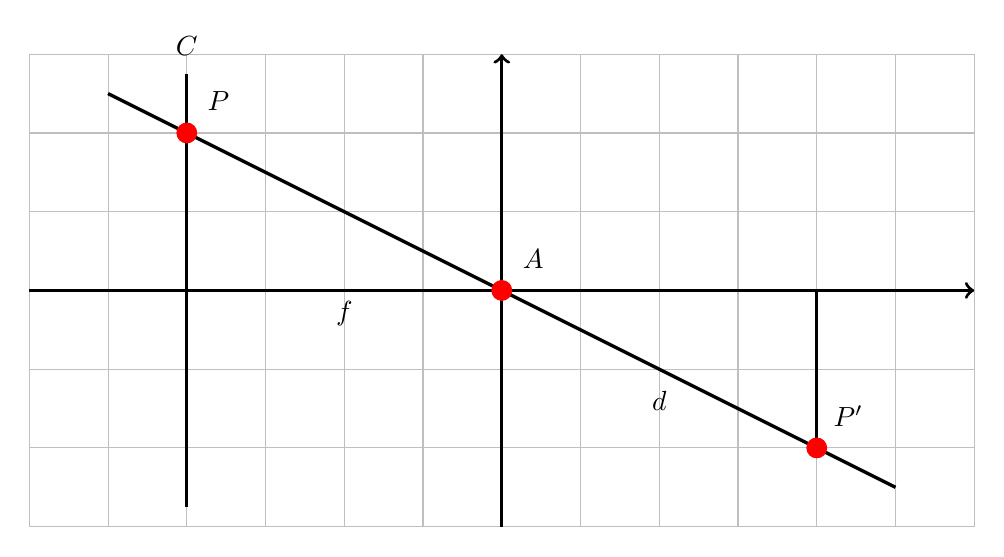
\begin{tikzpicture}
    % grid
    \draw [color=black!25] (0, 0) grid (12, 6);
    % x-axis
    \draw [very thick,->] (0, 3) -- (12, 3);
    % y-axis
    \draw [very thick,->] (6, 0) -- (6, 6);
    %
    \draw [very thick,-] (1, 5.5) -- (11, 0.5);
    %
    \draw [very thick,-] (2, 0.25) -- (2, 5.75);
    %
    \draw [very thick,-] (10, 3) -- (10, 1);
    % origin / aperture point
    \draw [color=red, fill=red] (6, 3) circle (0.125);
    \node at (6.4, 3.4) {$A$};
    %
    \draw [color=red, fill=red] (2, 5) circle (0.125);
    \node at (2.4, 5.4) {$P$};
    %
    \draw [color=red, fill=red] (10, 1) circle (0.125);
    \node at (10.4, 1.4) {$P'$};
    %
    \node at (4, 2.7) {$f$};
    %
    \node at (8, 1.6) {$d$};
    %
    \node at (2, 6.1) {$C$};
  \end{tikzpicture}
  \caption[The geometry of the pinhole camera model]{The geometry of the pinhole camera model, where $C$ is the camera image plane, $P$ is the 2D camera image pixel, $A$ is the camera aperture position, $f$ is the focal length of the camera, $P'$ is the 3D point in camera coordinate space and $d$ is the corresponding depth value from the depth image.}
  \label{fig:pinhole-camera}
\end{figure}

In order to calculate the pose, consisting of its position and orientation, and the dimensions of an object in 3D camera space, let $\overrightarrow{c}$ be the center of an object and $\overrightarrow{lb}$ the bottom left, $\overrightarrow{rb}$ the bottom right, $\overrightarrow{lt}$ the top left and $\overrightarrow{rt}$ the top right corners (see figure~\ref{fig:image-points}).

\begin{figure}[H]
  \centering
  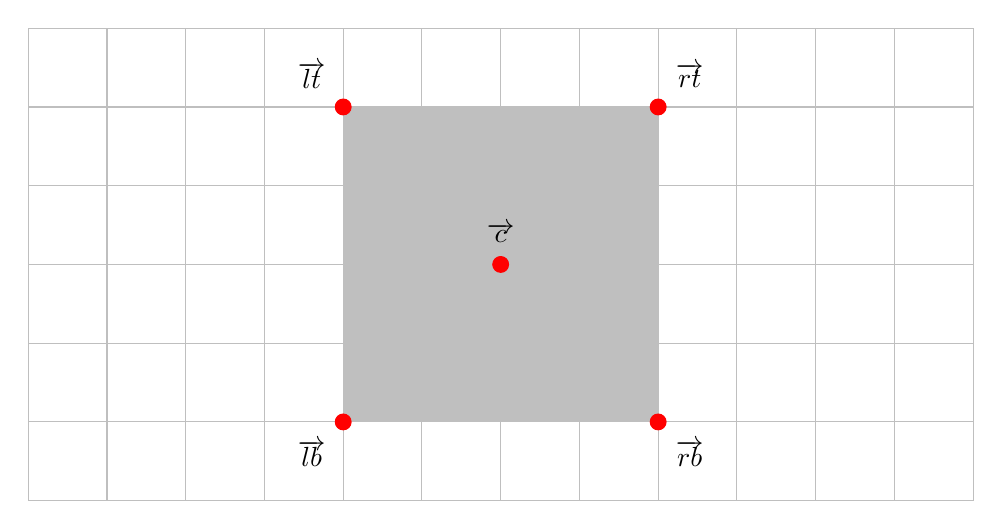
\begin{tikzpicture}
    % grid
    \draw [color=black!25] (0, 0) grid (12, 6);
    %
    \fill [color=black!25] (4, 1) rectangle (8, 5);
    %
    \draw [color=red, fill=red] (6, 3) circle (0.10);
    \node at (6, 3.4) {$\overrightarrow{c}$};
    %
    \draw [color=red, fill=red] (4, 1) circle (0.10);
    \node at (3.6, 0.6) {$\overrightarrow{lb}$};
    %
    \draw [color=red, fill=red] (8, 1) circle (0.10);
    \node at (8.4, 0.6) {$\overrightarrow{rb}$};
    %
    \draw [color=red, fill=red] (4, 5) circle (0.10);
    \node at (3.6, 5.4) {$\overrightarrow{lt}$};
    %
    \draw [color=red, fill=red] (8, 5) circle (0.10);
    \node at (8.4, 5.4) {$\overrightarrow{rt}$};
  \end{tikzpicture}
  \caption{Naming scheme for notable points of an object.}
  \label{fig:image-points}
\end{figure}

The \textbf{position} of an object is, by convention, located at its center (because the center is most likely to be hit by the laser sensor and therefore most likely to have a corresponding depth value). The center $\overrightarrow{c}$ of the object can be projected onto the camera image by applying the projection found in section~\ref{sec:impl-2Dpose}, then transformed into 3D camera coordinates as described above. If no depth value is available for this point, the object has to be discarded. \\

The \textbf{orientation}-vector of an object is an arbitrary, camera-facing vector that is orthogonal to two vectors that span the objects surface, for example its sides $\overrightarrow{w}$ and $\overrightarrow{h}$. Such a vector $\overrightarrow{n}$ is called a \textit{surface normal}. It can be determined by calculating the cross product of the surface vectors:
\begin{equation*}
  \overrightarrow{n} = \overrightarrow{w} \times \overrightarrow{h}
\end{equation*}
In order to get the sides of the object, at least three of its four corners (see figure~\ref{fig:image-points}) are needed. This guarantees, that either the top or the bottom
\begin{eqnarray*}
                  \overrightarrow{w} &=\ \overrightarrow{lt} - \overrightarrow{rt} \\
  \text{or}\qquad \overrightarrow{w} &=\ \overrightarrow{lb} - \overrightarrow{rb}
\end{eqnarray*}
and either the left or the right
\begin{eqnarray*}
                  \overrightarrow{h} &=\ \overrightarrow{lb} - \overrightarrow{lt} \\
  \text{or}\qquad \overrightarrow{h} &=\ \overrightarrow{rb} - \overrightarrow{rt}
\end{eqnarray*}
side can be calculated. The corner points are transformed into 3D camera space as described earlier in this section. How many of them then can actually be used depends on which have a corresponding depth value in the depth image.

The chances to get a usable depth value can be increased by using a point located between the center and the respective corner that is closer to $\overrightarrow{c}$, because such a point is more likely to have been observed by the laser sensor (points located closer to the sides have a tendency to ``fall of the edge''). This method does not change the resulting orientation vector, because the surface is perfectly flat. \\

The objects \textbf{dimensions} are the magnitudes of the previously calculated sides $\overrightarrow{w}$ and $\overrightarrow{h}$:
\begin{eqnarray*}
  \text{width}  &=\ |\overrightarrow{w}| \\
  \text{height} &=\ |\overrightarrow{h}|
\end{eqnarray*}


\section{Semantic Map}
\label{sec:impl-map}
Successfully recognized objects are stored in the semantic map, so other nodes (see Section~\ref{sec:impl-ros}) can find them when needed. As described in Section~\ref{sec:impl-perception}, the objects are published to a ROS topic by the perception. The semantic map subscribes to this topic and compares the received objects with those already memorised to distinguish between new additions and updates. \\

The architecture (Section~\ref{sec:arch-map}) defined multiple interfaces for the semantic map that allow other nodes access the memorized objects. These interfaces are implemented as ROS services. \\

This section deals not only with how the semantic map adds new information to its memory, but also with how it deals with noise and cleans up objects that changed their location. Furthermore, it explains how multiple objects of one type are evaluated, to provide other nodes with the best candidate.

\subsection{Memorising repeatedly confirmed and forgetting disappeared objects}
\label{sec:impl-memo}
3D poses published by the perception were perceived from a camera point of view. Because the camera moves, they have to be transformed to a fixed coordinate system before memorising them. The ROS package \textit{tf} is designed for this purpose: Current transformations are published to tf (e.q. by the robot running the proposed system), enabling it to resolve which one was valid at a specific point in time. Hence the tf package can be used to convert 3D poses between different coordinate system.

\begin{lstlisting}[caption=An example that shows how to use tf to transform a pose from one coordinate system to another.]
tf::TransformListener transform_listener;

// Coordinate system IDs
std::string camera_frame
  = "/head_mount_kinect_rgb_optical_frame";
std::string map_frame
  = "/map";

void map_2_camera(PoseStamped& pose_map,
                  PoseStamped& pose_camera)
{
  // Make sure transformation exists
  // at this point in time
  if(transform_listener.waitForTransform(
    map_frame,
    camera_frame,
    pose_map.header.stamp,
    ros::Duration(tf_timeout)
  )) {
    // Transform recognized camera pose to map frame
    transform_listener.transformPose(
      camera_frame,
      pose_map,
      pose_camera
    );
    pose_camera.header.stamp = ros::Time::now();
  }
}
\end{lstlisting}

After transforming an object to the fixed coordinate system, it is compared with those already stored in the semantic map. If an object of the same type already exists at the same position (within a certain range), the system assumes, that it is the same object. In this case, the existing object is updated by combining (basically calculating an average) their poses. Otherwise the new object is added to the semantic map.

As a range to determine if two object poses belong to the same object, its dimensions can be retrieved from the database (see Section~\ref{sec:arch-db}). The shorter side is the minimal distance between two objects unless they collide. \\

Section~\ref{sec:impl-2Dpose} dealt with precautions made to drop wrongly recognized objects. Still, some false positives might get through, but they should not end up in the semantic map. To this end, objects that are newly added need to be repeatedly recognized, otherwise they will be rejected (i.e. immediately removed again). When an object that has not yet been confirmed is updated, it gets flagged for confirmation. Every couple of seconds, a simple \textit{garbage collection} checks all memorised objects. The three cases that then may occur for each object are (1) the object has already been confirmed and is left untouched, (2) the object has been flagged for confirmation frequently enough and will be considered confirmed from now on, and (3) the object has not been flagged for confirmation frequently enough and is removed.

Similarly, objects can be flagged for removal, if they have already been confirmed, but are not recognized when they should be visible. The garbage collector transforms all objects back to the current camera coordinate system and checks if they are within the cameras opening angle and the range of the laser sensor, i.e. should be visible. If an object should be visible and was not updated since the last garbage collection, it gets flagged for removal. An object that has been flagged for removal to often gets deleted. This ensures, that objects are not stored forever, which is necessary to deal with objects that change their position.

\subsection{Improving the approximation of a 3D object pose by queueing multiple instances}
\label{sec:impl-queue}
Section~\ref{sec:impl-memo} briefly mentioned, that recognized objects which already exist in the semantic map are updated by combining their poses. The reason for this is, that the pose calculated by the perception (as described in Section~\ref{sec:impl-3Dpose}) is only an estimation that depends highly on the perspective, the matches from which the image-to-camera projection was derived, motion blur, etc. The estimation can be improved by using the calculations from multiple frames to approximate the real pose. \\

Multiple poses are combined by simply calculating their average. The average cannot just be calculated every time an object is recognized and memorized instead of the existing values, because one outlier could ruin the pose forever. Therefore, the semantic map uses first-in-first-out queues to keep the most recent poses for every object, enabling it to get an average from their actual values, not an accumulation of former calculations. Additionally, the poses are weighted by a ratio $|M|/|K|$, where $|M|$ is the number of matches the pose was derived from and $|K|$ is the number of keypoints found for the objects sample image (i.e. maximum number of matches the pose could have been derived from). This ensures that poor estimations do not ruin the average. \\

It should be mentioned here, that the database uses the same method to calculate an average for the dimensions of an object.

\subsection{Evaluating the relevance of memorized objects}
\label{sec:impl-eval}
The semantic map implements multiple interfaces (as described in Section~\ref{sec:arch-map}) through ROS services (see Section~\ref{sec:impl-ros}), to allow other nodes to access memorized objects. The system is not designed to find a specific object, but rather all objects that might be interesting in the future. It needs to be able to suggest the best candidates for a request, depending on the current situation, though. To this end, it implements an evaluation function, which prioritises objects by distance (closer objects are preferred, because they are faster reachable) and elapsed time since they were recognized (shorter periods are preferred, because it means an object is less likely to have changed its position). \\

In order to compare them, both aspects are evaluated separately and normalized in the process. The function should reflect, that recently detected objects are probably still there and that objects within a short range are located in the same section of the supermarket. It should then decline gradually and finally slowly approach $0$. Let
\begin{equation*}
  e(x) = 0.5\ -\ tan^{-1}(x * s -5)\ /\ \pi
\end{equation*}
be the evaluation function used for this purpose, then $\{0, 1\}$ is the range of $e(x)$. $s$ is the scaling factor, which is used to adjust $e(x)$, so that $x$ can have different ranges.

\begin{figure}[H]
  \centering
  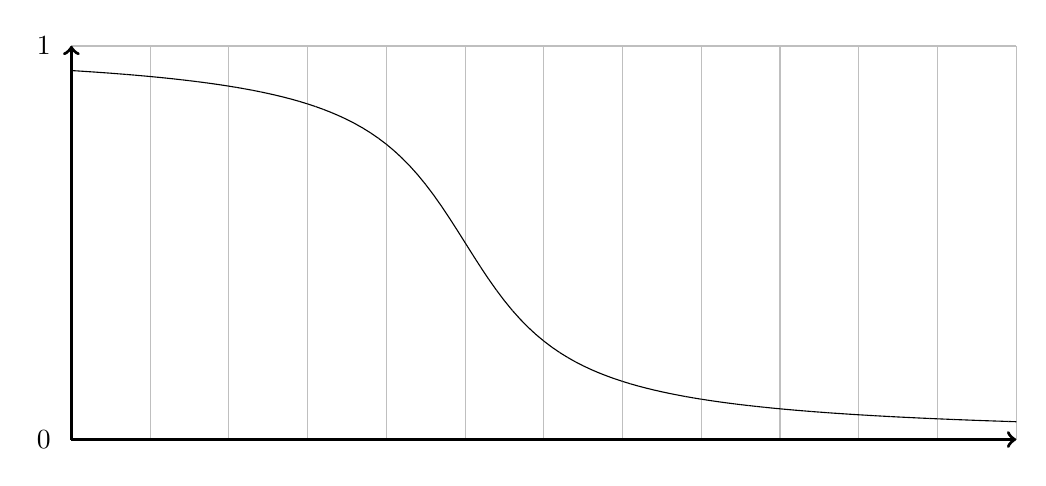
\begin{tikzpicture}[yscale=5]
    % grid
    \draw [color=black!25] (0, 0) grid (12, 1);
    % x-axis
    \draw [very thick,->] (0, 0) -- (12, 0);
    % y-axis
    \draw [very thick,->] (0, 0) -- (0, 1);
    % evaluation function
    \foreach \x in {0, 0.1, ..., 12} {
      \pgfmathsetmacro\tikzRad{180 / pi}
      \pgfmathsetmacro\tikzDeg{pi / 180}
      \pgfmathsetmacro\current{0.5 - atan(\x -5) / 180}
      \pgfmathsetmacro\next{0.5 - atan(\x+0.1 -5) / 180}
      \draw (\x, \current) -- (\x+0.1, \next);
    }
    %
    \node at (-0.35, 0) {$0$};
    \node at (-0.35, 1) {$1$};
  \end{tikzpicture}
  \qquad \\[-0.5ex]
  \label{fig:evaluation}
  \caption[Object relevance evaluation function.]{Visualisation of the evaluation function $e(x)$.}
\end{figure}

When evaluating the distance (in meters) between an object and the current camera position, it is defined as $s = 0.4$. As a result, $e(x)$ does only decline slowly for approximately $5m$ and starts to approach $0$ roughly between $x = 20$ and $x = 40$, which is appropriate for most supermarkets: A store with a sales floor of at least $400m^2$ is called a supermarket and the average supermarket has a sales floor of $800m^2$ \todo{Source}. Assuming square sales floors, distances in small to average supermarkets are around $20m - 40m$.

For the evaluation of the time (in seconds) that has passed since an object was seen for the last time, $s = 0.005$ is chosen as the scaling factor, meaning $e(x)$ stays high for about the first ten minutes and approaches $0$ between $x = 2000$ and $x = 3000$. This is sufficient for shopping scenarios that do not take longer than $30min - 60min$. \\

Both results are combined by simply calculating an average, but weighting distance higher than time:
\begin{equation*}
  e_{combinded}(x)\ =\ (2 \cdot e_{distance}(x) + e_{time}(x))\ /\ 3
\end{equation*}
$e_{combined}$ favours spatial over temporal distance, because going for close objects and not finding them is less of an issue than going for objects farther away and having to come all the way back.


\section{Visualization}
\label{sec:impl-viz}

\subsection{Visualising the Semantic Map in rviz}
ROS (see section~\ref{sec:impl-ros}) includes an application to visualize 3D objects and environments called \textit{rviz}. rviz can, among other things, draw basic shapes published by other nodes in the form of \textit{markers}. In this work, rviz is used to visualize the semantic map and along with the dimensions stored in the database. \\

For each object stored in the semantic map, several markers are published: A thin box, representing the object with all its attributes, position, orientation and dimensions; Three arrows, illustrating the objects axes (because the box alone cannot show its direction); And a text, showing the type of the object (in a different color - green - when the object is currently visible by the camera).

\todo{Image}
